\sub {

We now attempt to completely specify the space of ordered brackets, culminating in Corollary \ref{th:construct_order} and Theorem \ref{th:limit_order}.

We begin with a theorem that allows us to combine two smaller ordered brackets together into a larger ordered one by having the winner of one of the brackets slot into the lowest seed starting line of the other. This is depicted in Figure \ref{fig:ordered_bracket_staple}.

\fig{.95}{ordere_bracket_sum.png}{The Setup of Theorem \ref{th:order_bracket_sum}}{ordered_bracket_staple}

\theo{}{If $\A$ and $\B$ are $n$- and $m$-team ordered brackets, respectively, we can construct an $(n + m - 1)$-team oredered bracket by replacing the lowest seed in $\B$ with the entire bracket $\A$ (lowering the seed of each team in $\A$ by $m-1$).}{
Let $\C$ be the bracket formed by merging $\A$ and $\B.$ We divide proving that $\C$ is ordered into proving three substatements:
\begin{enumerate}
    \item For $i < j < m,$ $\P(t_i \textrm{ wins }\C) \geq \P(t_j \textrm{ wins }\C)$
    \item $\P(t_{m-1} \textrm{ wins } \C) \geq \P(t_m \textrm{ wins } \C)$
    \item For $m \leq i < j,$ $\P(t_i \textrm{ wins } \C) \geq \P(t_j \textrm{ wins } \C)$
\end{enumerate}
Together, these show that $\C$ is ordered.\\

We begin with the first substatement. Let $i < j < m.$ Then,
\begin{align*}
    \P(t_i \textrm{ wins }\C) &= \P(t_i \textrm{ wins }\B)\\
    &= \sum_{k=n}^{n+m-1} \P(t_i \textrm{ wins }\B \;\mid\; t_k \textrm{ wins } \A)\cdot \P(t_k \textrm{ wins } \A)\\
    &\geq \sum_{k=n}^{n+m-1} \P(t_j \textrm{ wins }\B \;\mid\; t_k \textrm{ wins } \A)\cdot \P(t_k \textrm{ wins } \A)\\
    &=\P(t_j \textrm{ wins }\B)\\
    &=\P(t_j \textrm{ wins }\C)
\end{align*}
The first and last equalities follow from the structure of $\C,$ and the inequality follows from $\B$ being ordered.\\

Now the second substatement.
\begin{align*}
    \P(t_{m-1} \textrm{ wins }\C) &= \P(t_{m-1} \textrm{ wins }\B)\\
    &\geq \P(t_{m} \textrm{ wins }\B \;\mid\; t_{m} \textrm{ wins }\A)\\
    &\geq \P(t_{m} \textrm{ wins }\B \;\mid\; t_{m} \textrm{ wins }\A) \cdot \P(t_{m} \textrm{ wins }\A)\\
    &= \P(t_{m} \textrm{ wins }\C)
\end{align*}
The equalities follow from the structure of $\C,$ and the first inequality follows from $\B$ being ordered.\\

Finally we show the third substatement. Let $m \leq i < j.$ Then,
\begin{align*}
    \P(t_i \textrm{ wins }\C) &= \P(t_i \textrm{ wins }\B \;\mid\; t_i \textrm{ wins } \A)\cdot \P(t_i \textrm{ wins } \A)\\
    &\geq \P(t_i \textrm{ wins }\B \;\mid\; t_i \textrm{ wins } \A)\cdot \P(t_j \textrm{ wins } \A)\\
    &\geq \P(t_j \textrm{ wins }\B \;\mid\; t_j \textrm{ wins } \A)\cdot \P(t_j \textrm{ wins } \A)\\
    &= \P(t_j \textrm{ wins }\C)
\end{align*}
The equalities follow from the structure of $\C$, the first inequality from $\A$ being ordered, and the second inequality from the teams being SST.\\

We have shown all three substatements, and so $\C$ is ordered.
}{order_bracket_sum}

\begin{corollary}{}{}
    If $\A = \bracksig{a_0; ...; a_r}$ and $\B = [b_0; ...; b_s]$ are ordered brackets, then $\C = \bracksig{a_0; ...; a_r + b_0 - 1; ...; b_s}$ is an ordered bracket as well.
\end{corollary}

We can then construct the set of brackets that we have thus far shown are ordered. We do this by starting with $\{\bracksig{1}, \bracksig{2; 0}, \bracksig{4; 0; 0}\}$ and then repeatedly applying the above theorem on the set to expand it. In other words,

\begin{corollary}{}{construct_order}
    Any bracket signature formed by the following process is ordered:
    \begin{enumerate}
        \item Start with the list $\bracksig{0}$ (note that this not yet a bracket signature).
        \item As many times as desired, prepend the list with $\bracksig{1}$ or $\bracksig{3; 0}.$
        \item Then, add 1 to the first element in the list, turning it into a bracket signature.
    \end{enumerate}
\end{corollary}

Corollary \ref{th:construct_order} uses the tools that we have developed so far to demark a set of brackets as ordered. Somewhat suprisingly, this set is complete: any bracket not reachable using the process in Corollary \ref{th:construct_order} is not ordered. To prove this we first show a lemma.

\lemm{}{
    If $\A$ is an $r$-round ordered bracket and two games are played in round $s$, then the winners of those games must play each other in round $s+1.$ Further, this must the only game of round $s+1$. 
}{
    Let $m$ be the number of teams that are still alive in $\A$ after round $s.$ Because $\A$ is proper, we know that if the bracket goes to chalk, $t_m$ will play $t_{m+1}$ in round $s$.\\

    Now, assume for contradiction that two games are played in round $s$ but the winners of those games do not play each other in the following round. So let $k<\ell$ such that, if the bracket goes to chalk, $t_k$ plays $t_\ell$ in round $s$, but the winner of that game doesn't play the winner of the $t_m$ game in round $s+1.$ In fact, let $k$ be the lowest such seed. Finally, let $i$ and $j$ be such that if the bracket goes to chalk, in round $s + 1$, $t_i$ will play $t_m$ and $t_j$ will play $t_k.$\\

    The situation so far (assuming all omitted games go chalk):
    \begin{center}
        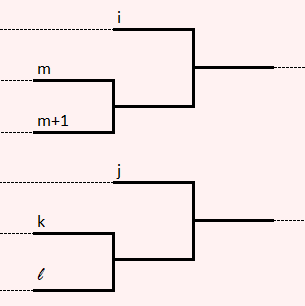
\includegraphics{images/two_must_play_ordered.png}
    \end{center}

    We can use $\A$'s properness to determine that $i < j < k < m < m + 1 < \ell.$\\

    Consider now the following SST set of matchups: games between two teams seeded $\ell + 1$ or higher are coin flips, games between $t_\ell$ and teams seeded between $t_{\ell+1}$ and $t_k$ are coin flips, and all other games are always won by the higher seed.\\

    Let's calculate the probability of $t_i$ and $t_j$ winning the tournament. $t_i$ will auto-win any games the have prior to round $s+1$, and then have to win $r - s$ coin flips in order to win the tournament. This happens with probability $0.5^{r-s}.$\\

    $t_j$ will also win all of its games prior to round $s+1$, also has to win a coin flip for each games in round $s+2$ or later. For round $s+1$, however, half the time $t_j$ will be matched up with $t_k$, which is a coin flip, but half the time they will be matched with $t_k$, which is an auto-win. Thus, $t_j$ will win the tournament with probability $0.75(0.5)^{r-s-1}.$\\

    Therefore, $t_j$ has a better chance of winning the tournament than $t_i$ does, despite $t_i$ being higher seeded, so $\A$ is not ordered, completing the contradiction. Thus if two games are played in round $s$, the winners of those games must play each other in round $s+1.$\\

    This immediately implies that at most two games can be played in each round of an ordered bracket.\\
    
    Finally, we know that this can be the only game played in round $s+1$ because if there was another game, it would have to be between two teams that are higher-seeded than the two teams who won in the previous round, meaning that round violated condition (2).
}{two_must_play}

And now the main theorem,

\theo{}{
    The only ordered brackets are those described by Corollary \ref{th:construct_order}.
}{
    Corollary \ref{th:construct_order} describes all proper brackets in which each round either has only game, or has two games but is immediately followed by a round with only one game. A proper bracket not described by Corollary \ref{th:construct_order} would thus have to include a round with two or more games followed by another round with two or more games, violating Lemma \ref{th:two_must_play}.
}{limit_order}

Theorem \ref{th:limit_order} is both exciting and disapointing. On one hand, it means that Corollary \ref{th:construct_order} fully describes the set of ordered brackets, making it easy to, e.g., check whether a given bracket is ordered or not. On the other hand, it means that in an ordered bracket at most three teams can be introduced each round, so the length of the shortest ordered bracket on $n$ teams grows linearly with $n$ (rather than logarithmically as is the case for proper brackets). If we want a bracket on many teams to be ordered, we risk forcing lower-seeded teams to play large numbers of games, and we only permit the top seeded teams to play a few. For example, if the shortest ordered bracket that could've been used in the 2022 NCAA Women's Basketball Wichita Region is $\bracksig{4; 0; 3; 0; 3; 0; 3; 0; 3; 0; 0},$ which is played over a whopping ten rounds.

\fig{.475}{ordered_sixteen.png}{The Shortest Sixteen-Team Ordered Bracket}{}

Because of this, few leagues uses ordered brackets, and those who do usually have so few teams that every proper is bracket (the 2023 College Football Playoffs, for example.) Even the Korean Baseball Organization League, which uses a somewhat unconventional $\bracksig{2; 1; 1; 1; 0},$ only sends five teams to the playoffs, and again every five-team proper bracket is ordered. If the KBO League ever expanded to the six-team bracket $\bracksig{2; 1; 1; 1; 1; 0},$ we would have a case of an ordered bracket being used instead of a proper non-ordered bracket on the same number of teams.
}